\section{Introduzione}
L'heap è una regione di memoria assegnata ad un processo, vedi Figura~\ref{fig:proc}, per dati la cui esistenza o dimensione non è conosciuta a tempo di compilazione. A differenza dello stack, la vita di un'allocazione non dipende dalla procedura o dallo stack frame corrente. Questa memoria, infatti, è globale, quindi può essere acceduta e modificata da qualunque parte del programma, in maniera indiretta, per mezzo di un puntatore. 

\begin{figure}[b]
	\centering
	\label{fig:proc}	
	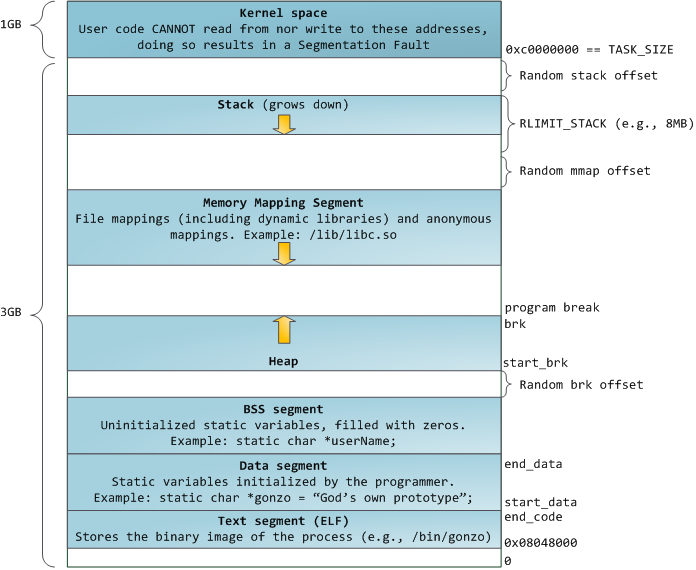
\includegraphics[width=10cm]{process_layout}
	\caption{Processo in memoria}
\end{figure}

La libreria standard del linguaggio C consente di interagire con l'heap mediante due funziono:
\begin{lstlisting}[style=CStyle]
void* malloc(size_t size)
\end{lstlisting}
che alloca in heap uno spazio di dimensione \verb+size+ byte, e
\begin{lstlisting}[style=CStyle]
void free(void* p)
\end{lstlisting}
che dealloca dall'heap la zona di memoria puntata da \verb+p+, precedentemente allocata da \verb+malloc+.

Esistono una serie di regole, di cui è responsabile il programmatore, che se rispettate consentono di evitare bug:
\begin{enumerate}
\item liberare una zona di memoria con \verb+free+ ottenuta da una \verb+malloc+
\item non usare \verb+free+ su una zona di memoria più di una volta
\item assicurarsi di non sovrascrivere zone di memoria che eccedono la memoria richiesta dalla \verb+malloc+, per evitare \emph{heap overflow}.
\end{enumerate}